\chapter{Lien entre les noeuds}\label{chapter:lien}
\label{sec:prerequis}

	\section{Lien prélude-noeud}
		Ce lien est très important. Il permet à l'utilisateur d'utiliser toutes les options possible dans la barre de menu, dans l'onglet "\textit{Livre}". Cela permet d'indiquer le premier noeud qui va être lu, après le prélude. Ce noeud peut être tracé grâce au mode 
\includegraphics[height=10pt]{img/modePreludeNoeud.png} même si le prélude n'est pas complété. En effet, le joueur va alors avoir un personnage préétabli.
		Une fois le mode selectionné, un simple clique sur un carré est nécessaire. Si l'utilisateur veut changer le premier noeud, le même mode 
\includegraphics[height=10pt]{img/modePreludeNoeud.png} doit être sélectionné, et le même procédé est nécessaire.

	\section{Lien entre les noeuds}
		Ces liens permettent de relier un paragraphe à un autre paragraphe grâce à un choix. Ce lien ne peut pas commencer sur un noeud terminal, ni sur le prélude. Tant que tout les liens ne sont pas créés, il est impossible de jouer, ni d'estimer la difficulté.\\

		Pour tracer ce lien, le mode 
\includegraphics[height=10pt]{img/modeLien.png} est requis. L'utilisateur doit alors cliquer sur un premier noeud, puis sur un deuxième. Ce noeud peut être le même afin de laisser la liberté de créer une boucle si necessaire.
		Si le permier clique n'était pas voulu, un simple clique dans la zone vide d'édition est requis pour annulé le premier clique.\\

		Une fois ce lien trâcé, une boite de dialog apparait. Elle contient un texte qui s'affichera lors de l'affichage de tout les choix, deux champs de texte de gain/perte de point de vie et de monnaie, ainsi que d'un onglet contenant les prérequis. Une coche est également disponible permettant de prendre toujours ce choix automatiquemenent.
		Ces prérequis permettent à l'utilisateur de créer des choix où il est possible d'y accèder que si certains objets/compétences sont possédés par le joueur.
		Pour cela, un bouton 
\includegraphics[height=10pt]{img/ajouterBouton.png} permet de créer des listes de prérequis. Comme par exemple, le joueur doit posséder l'épée "Excalibur" ainsi que le bouclier "Pavois" \textbf{ou} trois d'argent ainsi que la compétence "Boule de feu" et l'épée "Excalibur".
		Pour l'ajout de ces items/monnaie/compétences, c'est le même procédé que \ref{subsubsection:compétences} et \ref{subsubsection:Item/Shop}.\\

		Tout les champs des liens, sauf le champ contenant le texte du choix (\textit{Texte}), ne peut contenir des lettres et ne peut être vide. L'utilisateur ne peut valider que si ces conditions sont remplis. S'il décide d'annuler, toutes les modifications seront perdu.\\

		\subsection{Lien noeud combat}\label{subsection:lienCombat}
			\begin{minipage}{0.70\textwidth}
				Si le premier noeud cliqué est un noeud de combat, une liste déroulante "Type de lien" est présente dans l'onglet lien. Cela permet donc de définir, par rapport au déroulement du combat, le lien qui sera parcouru. Tout les types de lien ne sont pas obligatoire pour jouer au jeu, mais cela va alors conduire le joueur obligatoirement sur un noeud terminal de défaite, même si le combat a été gagné.
			\end{minipage}
			\hfill
			\begin{minipage}{4cm}
				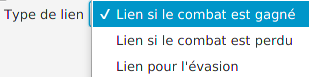
\includegraphics[width=4cm]{img/lienCombat.png}
			\end{minipage}

		\subsection{Lien noeud aléatoire}\label{subsection:lienAléatoire}
			Si le premier noeud cliqué est un noeud aléaoire, un champ de texte permet de renseigner le nombre chance pour aller vers ce lien. L'utilisateur pourra alors laisser libre court à son imagination afin de créer des chemins aléatoire.\\

			\begin{figure}[H]
				\centering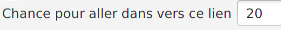
\includegraphics[width=4cm]{img/lienAleatoire.png}
			\end{figure}


	\section{Modification des liens}
		Une modification des liens se fait grâce au mode 
\includegraphics[height=10pt]{img/modeSelected.png}. Un simple double clique sur le lien est necessaire pour modifier ce dernier.

	\section{Suppression des liens}
		Ces liens, sauf le lien du prélude, peuveut être supprimés à l'aide du mode 
\includegraphics[height=0.4cm]{img/modeSupression.png}. Un simple clique sur le lien est alors necessaire. Une boite de dialog va alors s'ouvrir permettant de vérifier si l'utilisateur est bien sûr de son action.
		Si c'était un lien de combat, le type de ce lien est alors libre.
